\chapter{Appendix}
\label{chp:appendix}

\section{Printing}
\label{sec:Printing}

The exported PDF file(s) with the attenuation masks can directly be printed with any device that supports transparencies.
The attenuation layers for this project have been printed with an old HP Photosmart C5180 ink-jet printer.
The built-in photo-printing mode turned out to work best, but all automatic image enhancement settings (e.g. red-eye removal) must be turned off in the advanced settings.
Also, ink-jet printers require special types of transparencies that have a rough surface such that the ink can hold on to the sheet.

\section{Backlight Fabrication}
\label{sec:backlight_fabrication}

For an optimal viewing experience, a uniform backlight is needed to place behind the glass plates which hold the printed transparencies.
LEDs are the optimal choice for a simple white backlight: They are small sized, power saving, affordable and don't produce a lot of heat when turned on.
The ones used for this build are average, consumer grade quality LEDs bought on Amazon.
A detailed specification of the product is given in table~\ref{tbl:LED_specs}.
\begin{table}[tb]
	\centering
	\begin{tabular}{| l | l |}
		\hline
		LED Chip					& SMD 5050 \\
		\hline
		Electric current			& 12V DC \\
		\hline
		Color 						& Cold white \\
		\hline 
		Color temperature 			& 6000 Kelvin \\ 
		\hline  
		Luminous flux 				& 4500 Lumen \\ 
		\hline
		Emission angle				& 120$^\circ$ \\
		\hline 
		Power consumption			& 60 Watt \\
		\hline
		Average lifespan			& 50000 hours \\
		\hline
	\end{tabular} 
	\caption[LED specification]
			{Specification of LEDs used for the backlight.}
	\label{tbl:LED_specs}
\end{table}
A five meter long and 10 mm wide LED strip is cut into pieces of 15 cm length, each having nine LEDs.
These smaller strips are placed next to each other and glued onto a wooden plate forming the base for the backlight.
Corresponding ends of the strips are reconnected by soldering small pieces of wire onto the contacts of the strips.
For an easier soldering process and to reduce the risk of an electrical short, the strips are alternately offset by a small amount as shown in figure~\ref{fig:look_inside_backlight_2}.
\begin{figure}[tb]
	\subcaptionbox{\label{fig:all_three_backlights}}{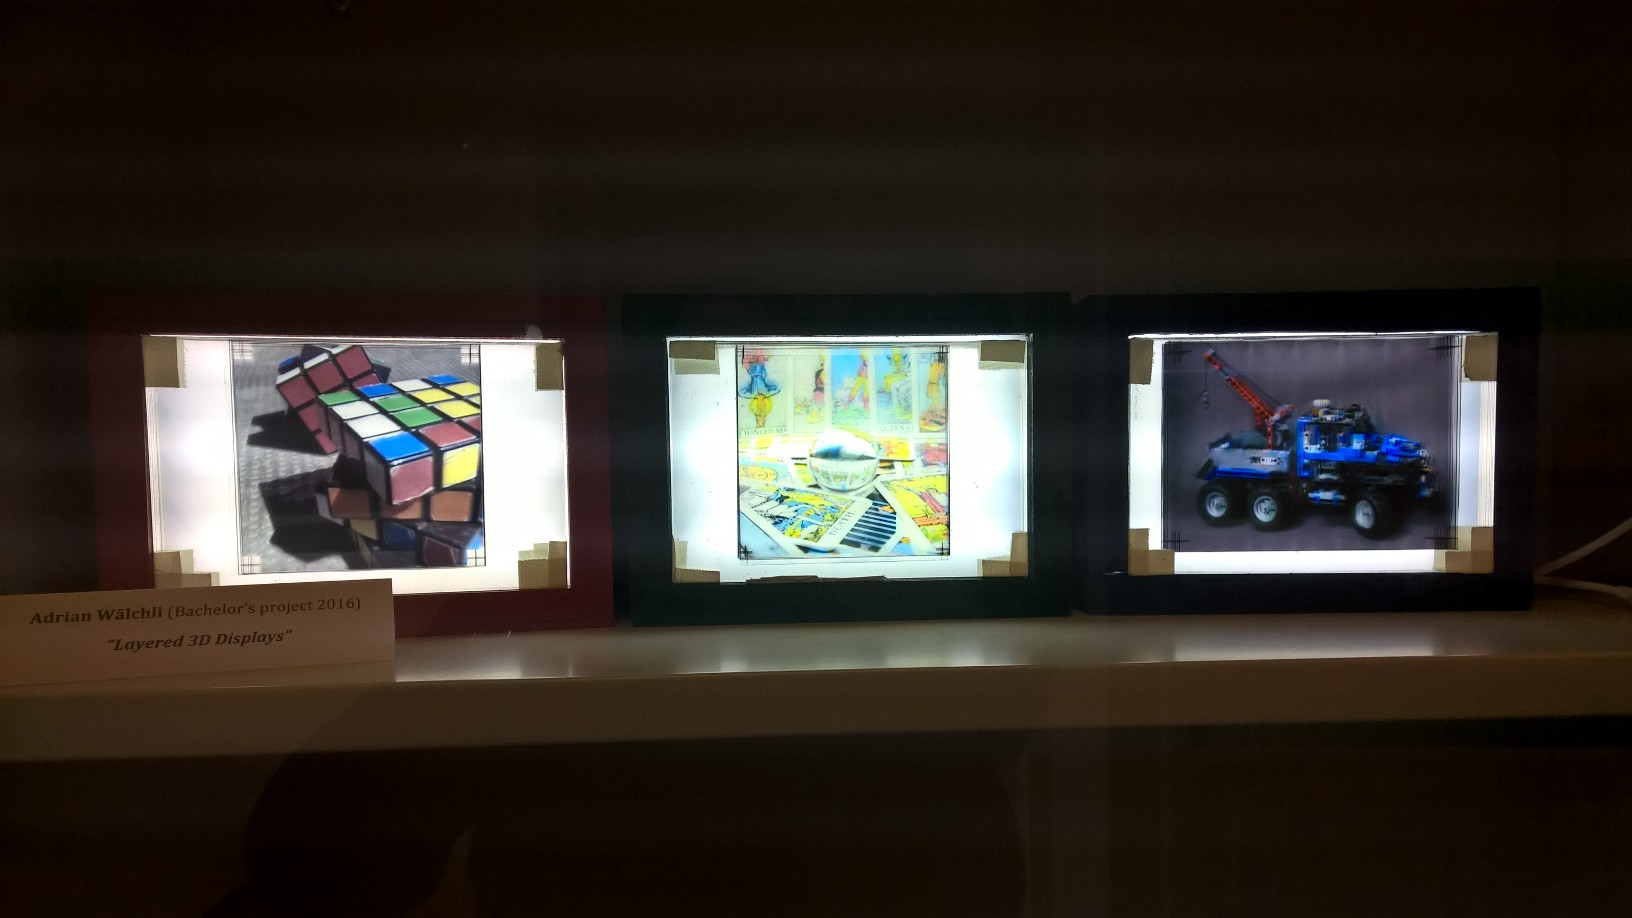
\includegraphics[trim={2cm 10cm 3cm 9cm}, clip, width = \linewidth]{../Figures/hand_craft/all_displays_on.JPG}}\hfill%
	
	\vspace{0.15cm}
	
	\subcaptionbox{\label{fig:look_inside_backlight_1}}{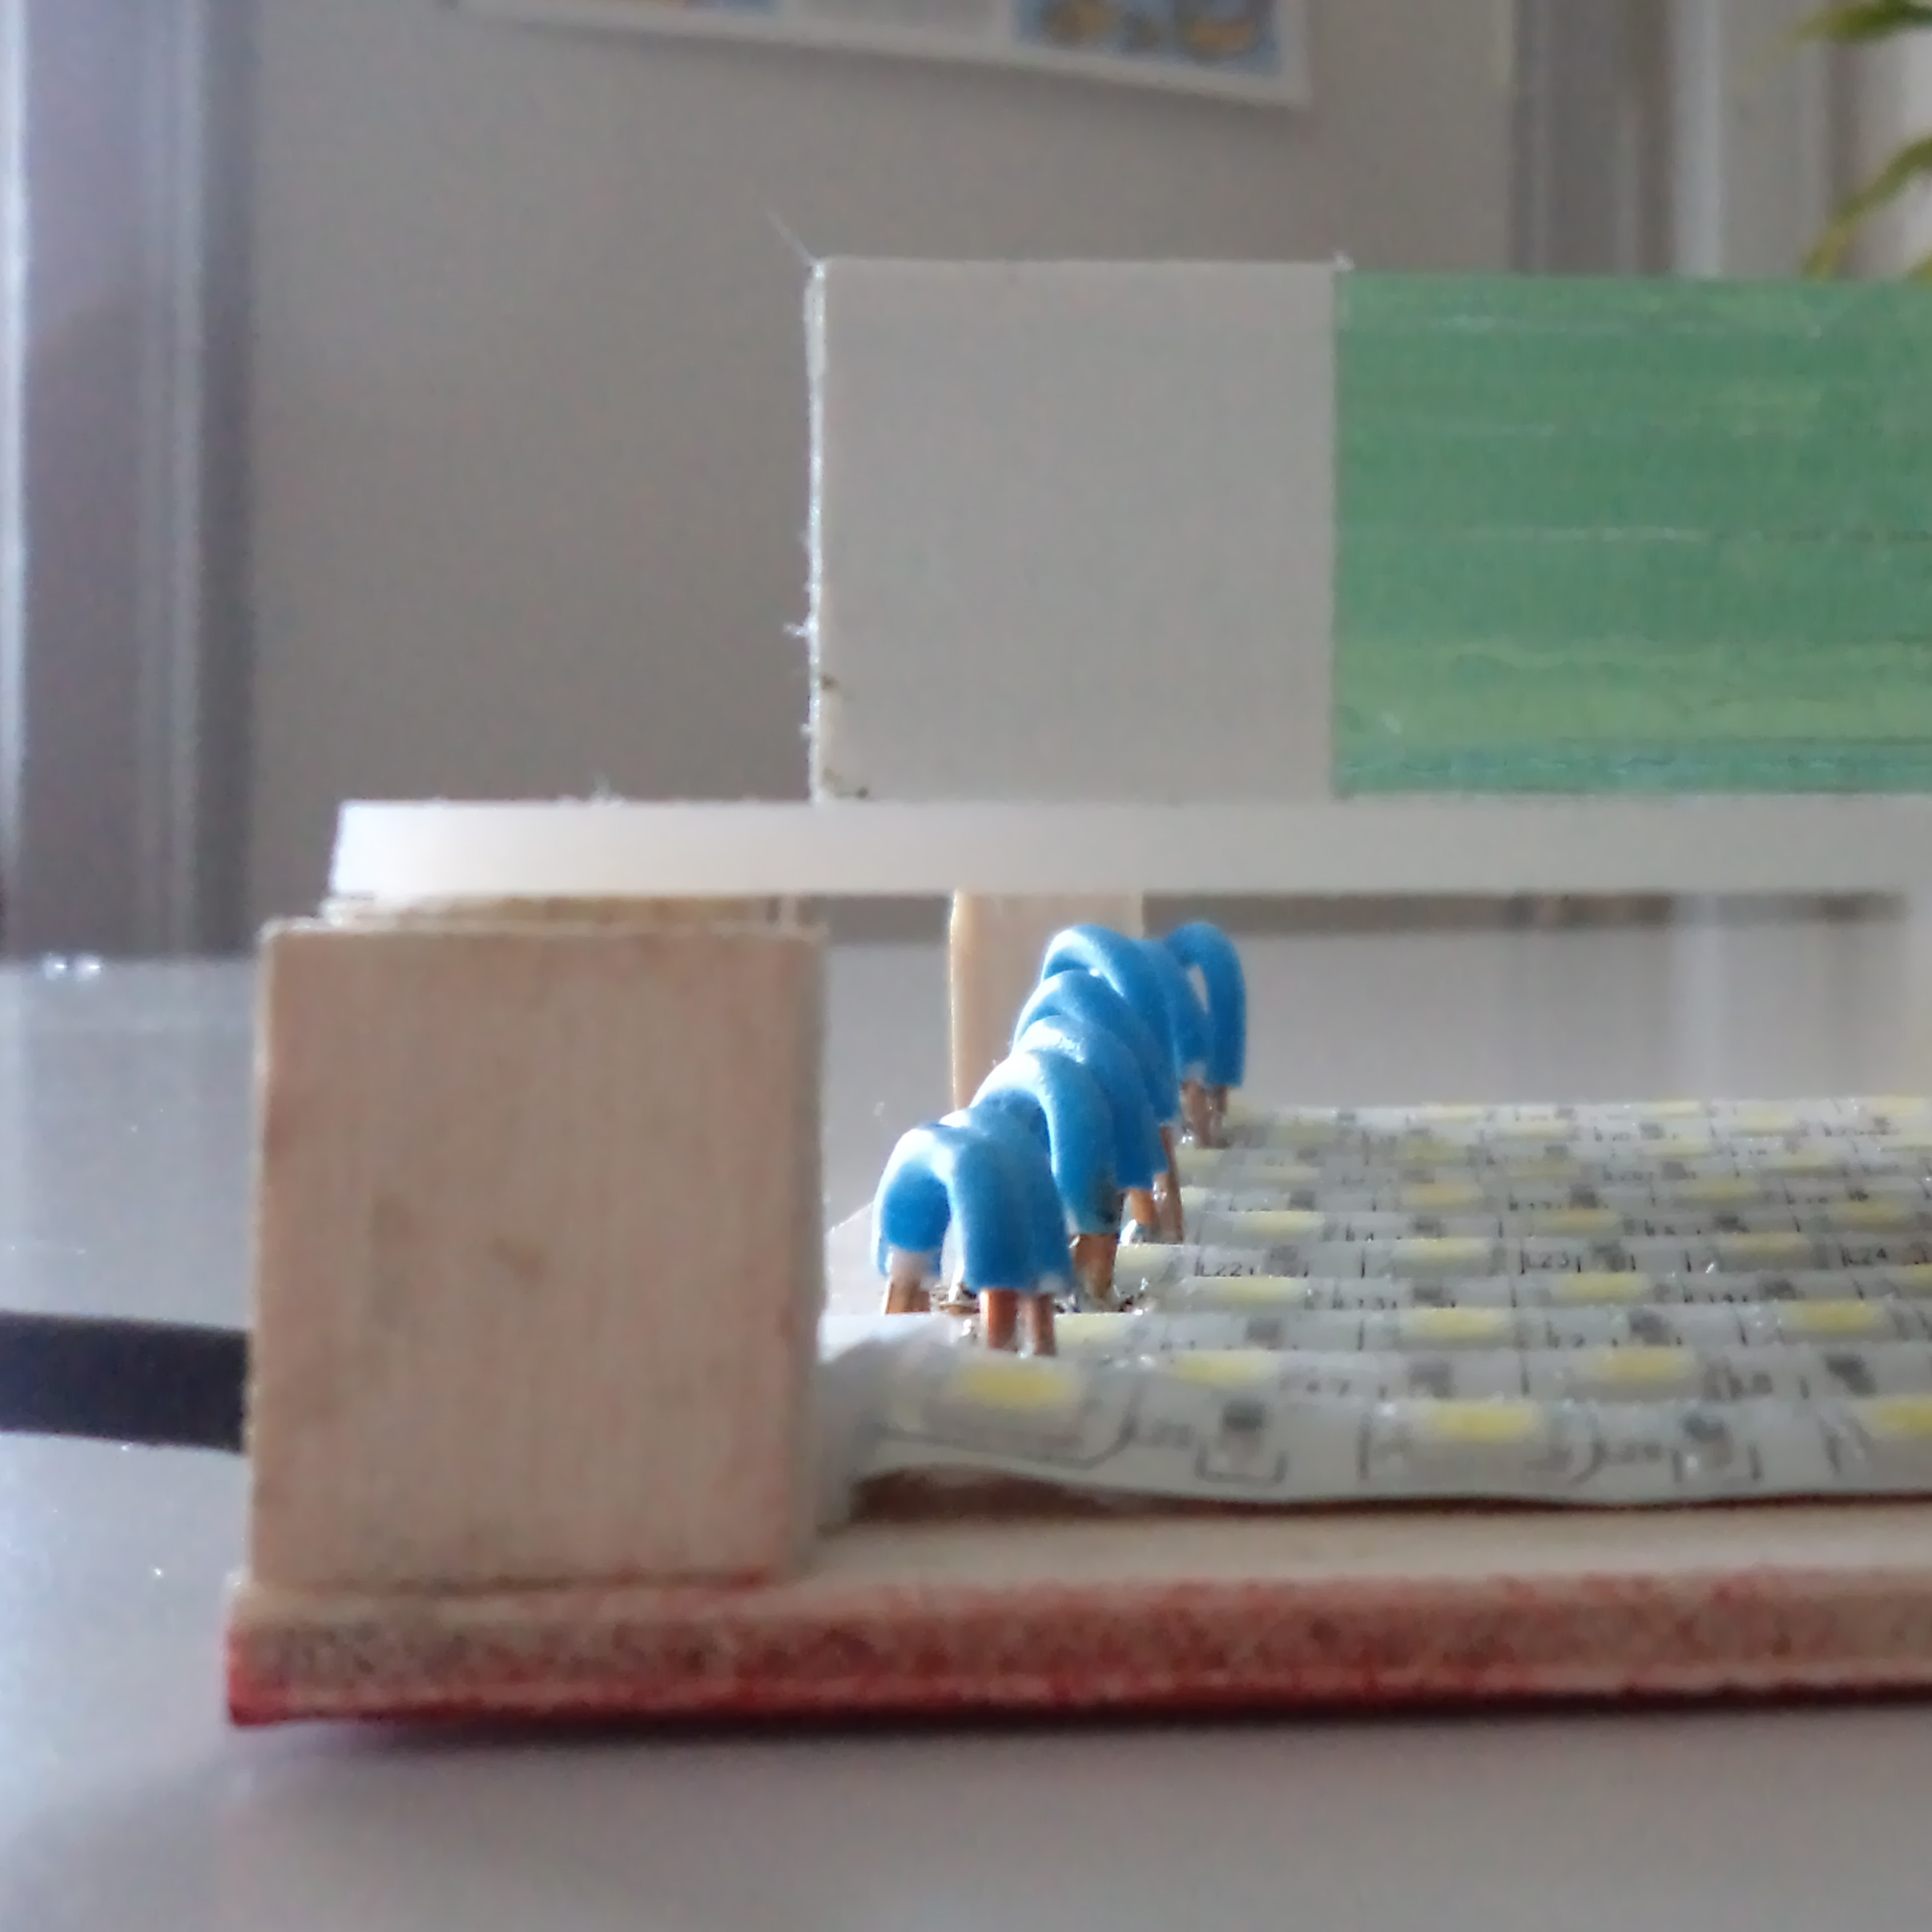
\includegraphics[width = 0.45\linewidth]{../Figures/hand_craft/display_frame_removed_cropped.jpg}}\hfill%
	\subcaptionbox{\label{fig:look_inside_backlight_2}}{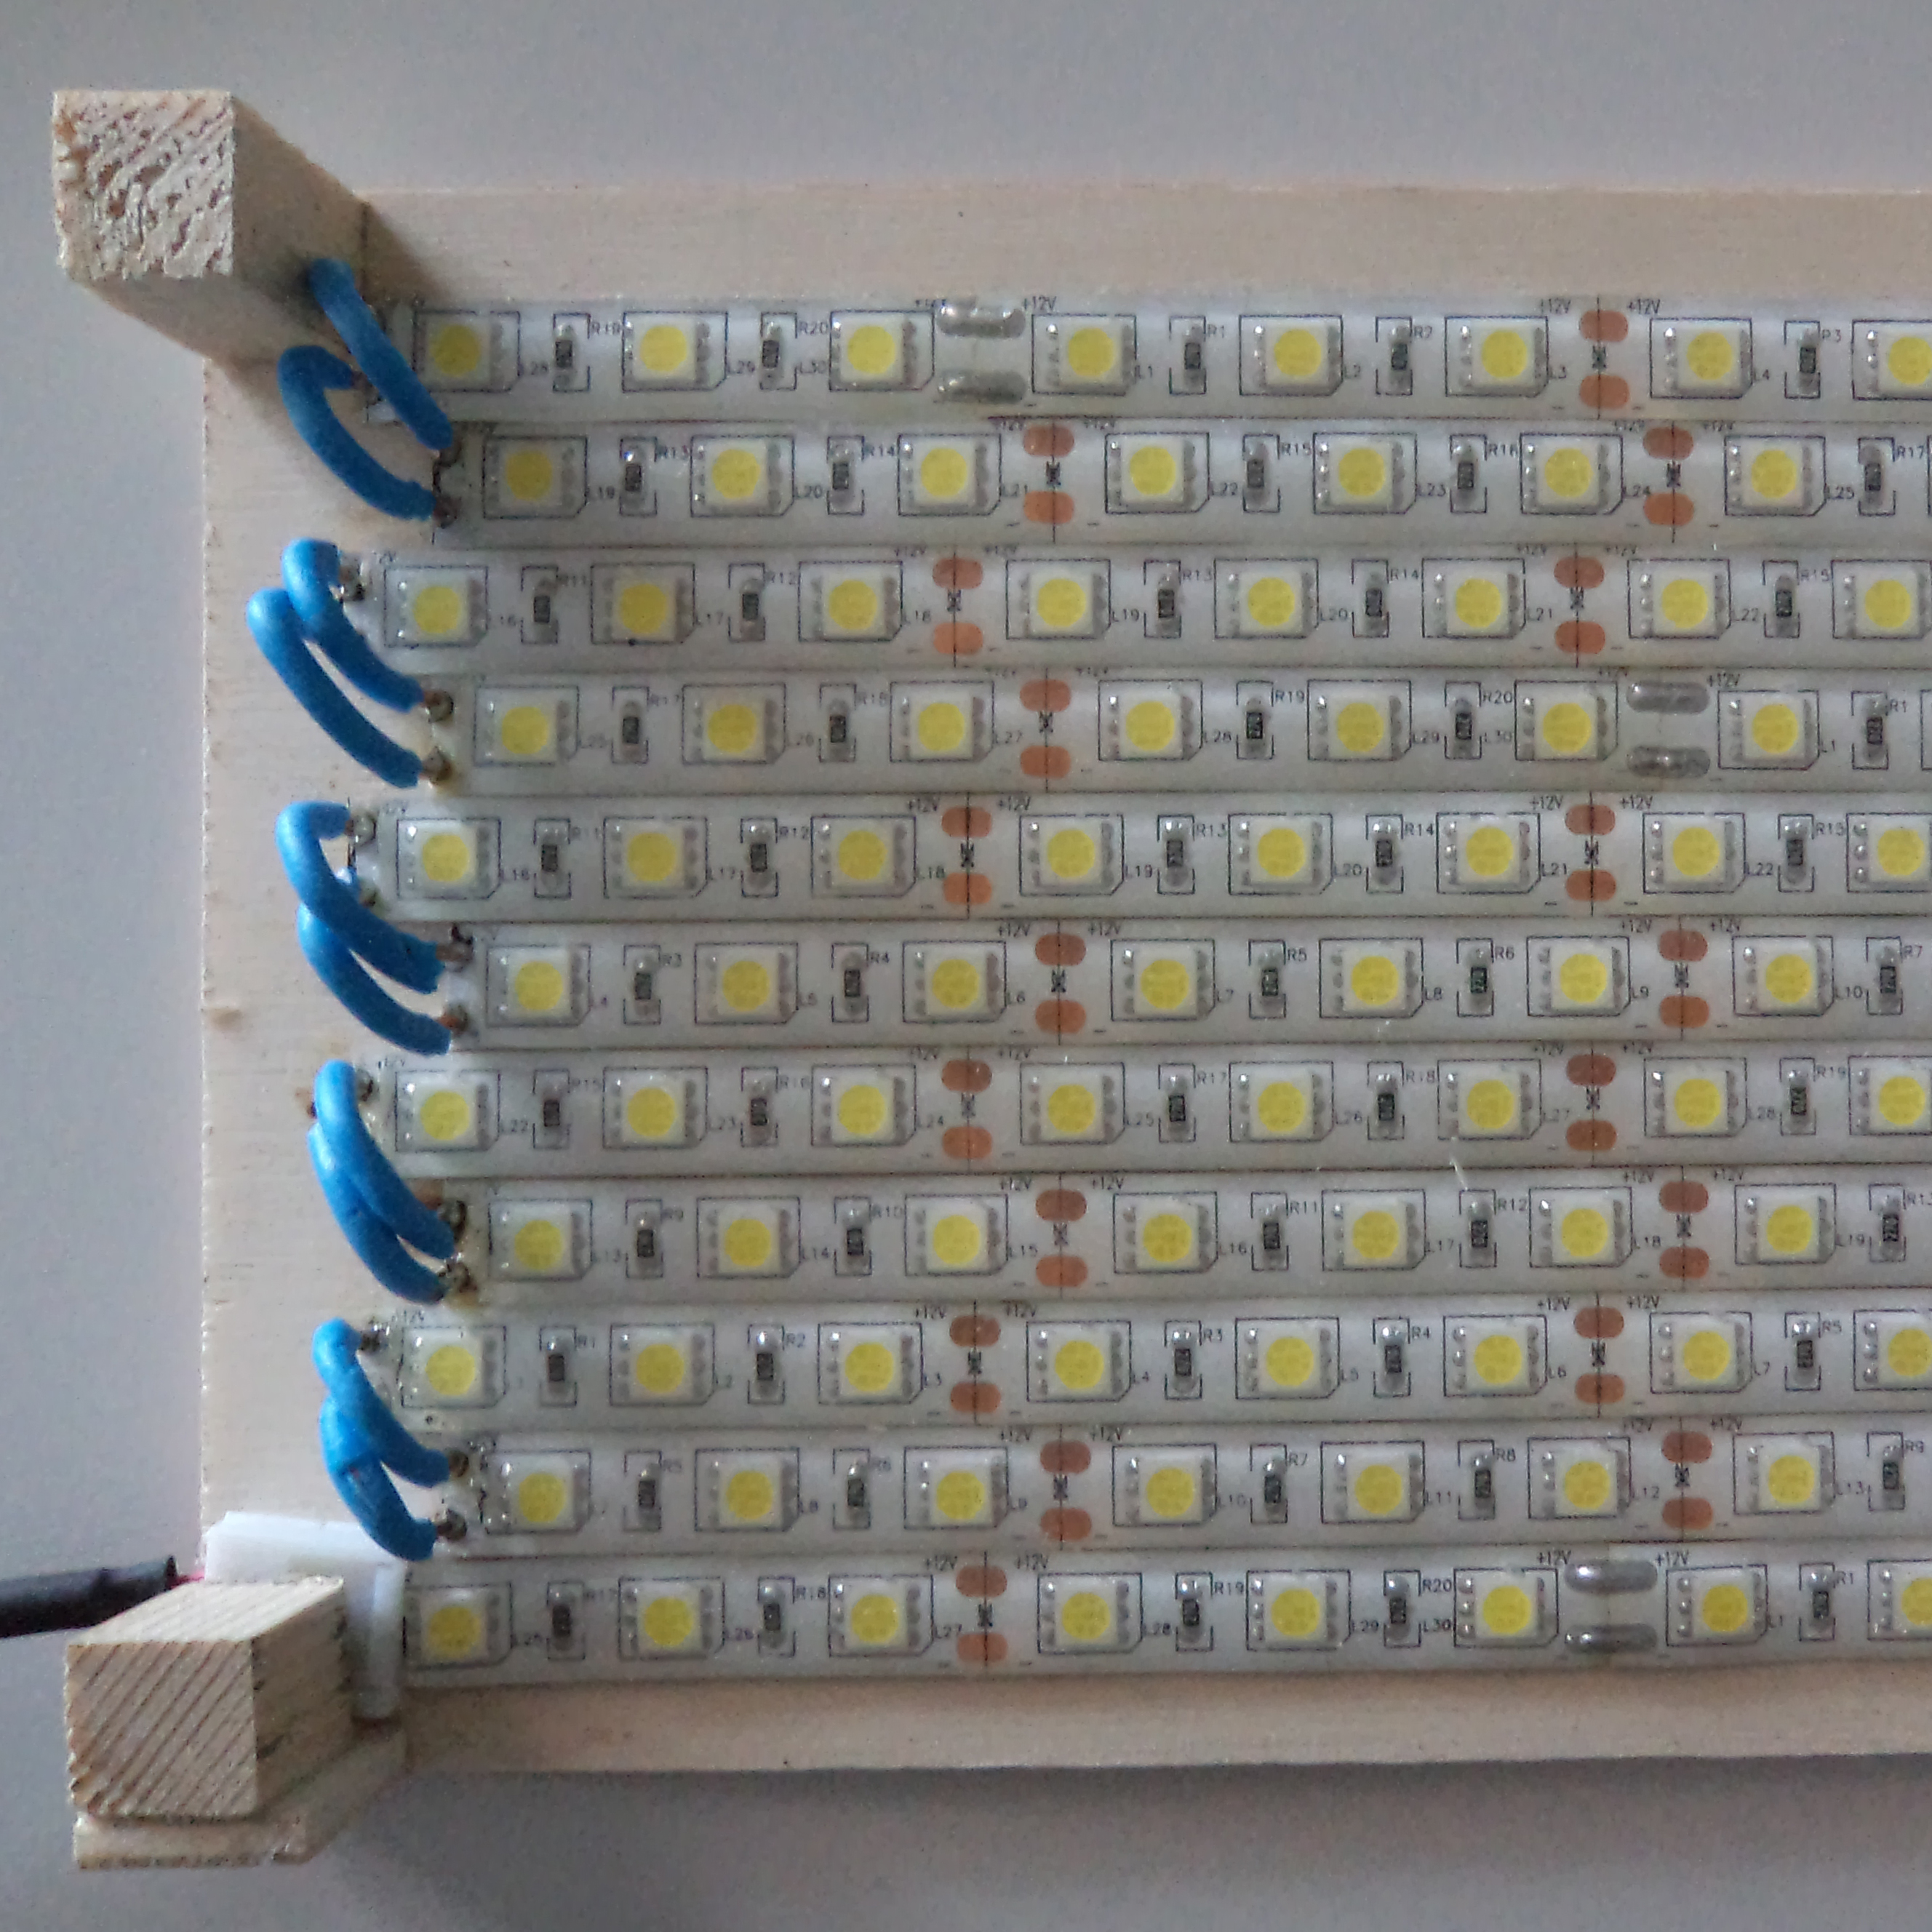
\includegraphics[width = 0.45\linewidth]{../Figures/hand_craft/raw_backlight_from_top_cropped.jpg}}
	\caption[Handcrafted backlights for the attenuation displays]
			{(a) Three fully assembled displays with backlight.
			 (b) Close up of the inside with the outer frame removed.
				 Top to bottom: Glass plates holding attenuation layers, diffusion plate, LED grid.
			 (c) Close up of the LED grid with the diffuser removed.}
	\label{fig:hand_crafted_backlight}
\end{figure}
A connector for the power supply is mounted on one end of the strip.
Wooden stand-offs glued to the base hold the diffuser plate 17 mm above the LEDs.
The diffuser is simply a white, milky acrylic plate from a hardware store, cut to the right size.
Finally, the build is concluded with a wooden frame covering the LEDs and wires and holding the glass plates in place.
The frame has a diagonal of 23 cm, is 5 cm thick and is painted with a color varnish to protect the wood from scratches and to beautify the product.

A total of three backlights were produced for this project.
All three displays are powered by a 12V/6A DC power supply.
The set also includes a remote control to turn the displays on and off or to adjust the brightness level.

\section{More Simulated Projections}
\label{sec:simulated_projections}

The following pages show simulated projections from various scenes displayed with the attenuation display.
All the examples here have display parameters that correspond to the displays shown in figures~\ref{fig:glass_display} and~\ref{fig:hand_crafted_backlight}.
Five layers are equally spaced to form a 1.6 cm thick stack.
The baseline has been manually adjusted such that the desired depth range is approximately within the displays depth of field.
Each simulated view is labeled with an index $(i, j)$ that corresponds to the location of the virtual camera on the \mbox{$(u, v)$-plane} where $i$ denotes the vertical placement from top to bottom and $j$ denotes the horizontal placement from left to right.
The images below each simulation show the per-pixel \mbox{RMSE} over the three color channels.
High error is visualized with yellow and red color and bluish colors indicate low error.

\begin{figure}[htb]
	\subcaptionbox*{(1,1)}{
\includegraphics[height = 3.5cm]{../Figures/simulated_views/knights_tiles3x3x256x256_overlap0.5_5layers_resolution9x9x512x512_SART_50iter/Reconstruction_of_view_(1,1).png}}\hfill%
	\subcaptionbox*{(1,5)}{
\includegraphics[height = 3.5cm]{../Figures/simulated_views/knights_tiles3x3x256x256_overlap0.5_5layers_resolution9x9x512x512_SART_50iter/Reconstruction_of_view_(1,5).png}}\hfill%
	\subcaptionbox*{(1,9)}{
\includegraphics[height = 3.5cm]{../Figures/simulated_views/knights_tiles3x3x256x256_overlap0.5_5layers_resolution9x9x512x512_SART_50iter/Reconstruction_of_view_(1,9).png}}
	
	\vspace{0.15cm}
	
	\subcaptionbox*{(1,1)}{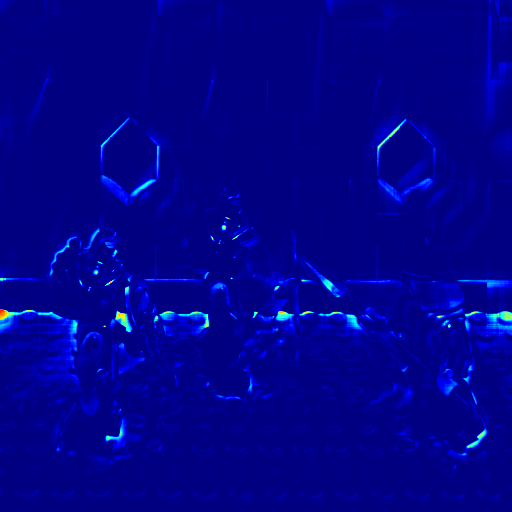
\includegraphics[height = 3.5cm]{../Figures/simulated_views/knights_tiles3x3x256x256_overlap0.5_5layers_resolution9x9x512x512_SART_50iter/MSE_for_view_(1,1).png}}\hfill%
	\subcaptionbox*{(1,5)}{
\includegraphics[height = 3.5cm]{../Figures/simulated_views/knights_tiles3x3x256x256_overlap0.5_5layers_resolution9x9x512x512_SART_50iter/MSE_for_view_(1,5).png}}\hfill%
	\subcaptionbox*{(1,9)}{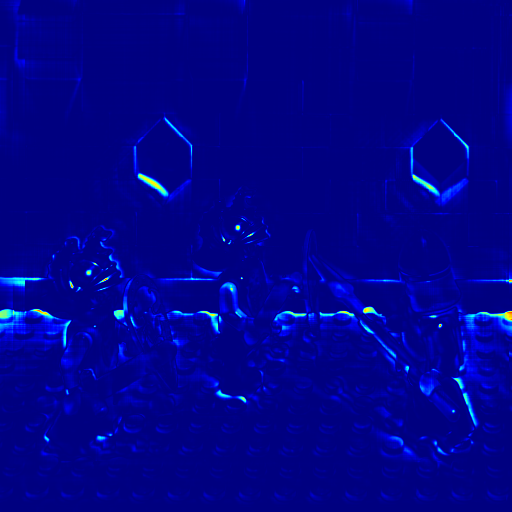
\includegraphics[height = 3.5cm]{../Figures/simulated_views/knights_tiles3x3x256x256_overlap0.5_5layers_resolution9x9x512x512_SART_50iter/MSE_for_view_(1,9).png}}
	
	\vspace{0.15cm}
	
	\subcaptionbox*{(5,1)}{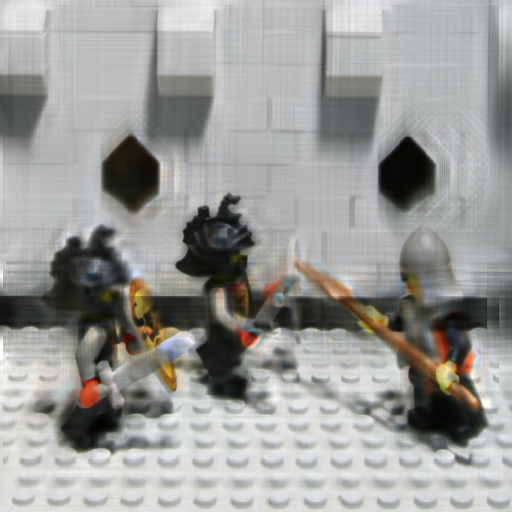
\includegraphics[height = 3.5cm]{../Figures/simulated_views/knights_tiles3x3x256x256_overlap0.5_5layers_resolution9x9x512x512_SART_50iter/Reconstruction_of_view_(5,1).png}}\hfill%
	\subcaptionbox*{(5,5)}{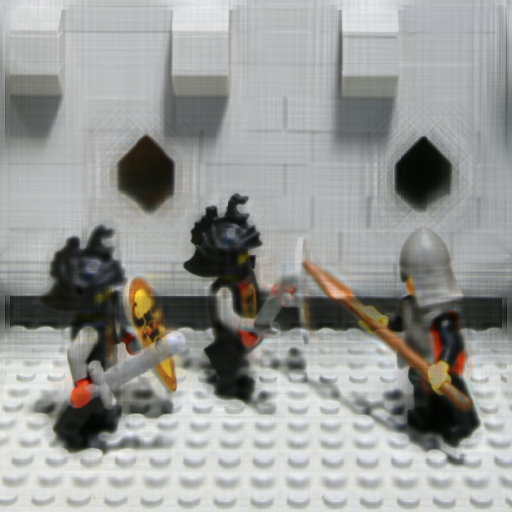
\includegraphics[height = 3.5cm]{../Figures/simulated_views/knights_tiles3x3x256x256_overlap0.5_5layers_resolution9x9x512x512_SART_50iter/Reconstruction_of_view_(5,5).png}}\hfill%
	\subcaptionbox*{(5,9)}{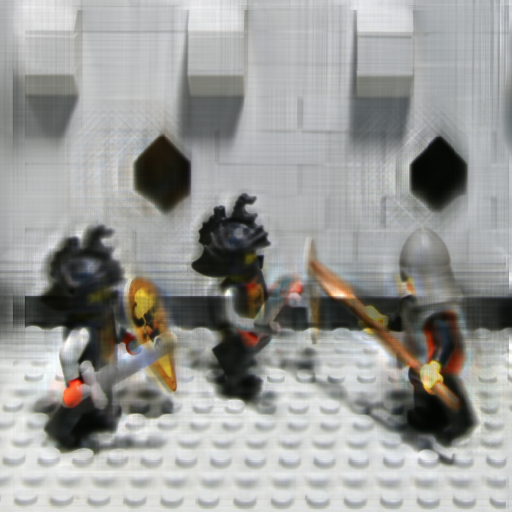
\includegraphics[height = 3.5cm]{../Figures/simulated_views/knights_tiles3x3x256x256_overlap0.5_5layers_resolution9x9x512x512_SART_50iter/Reconstruction_of_view_(5,9).png}}
	
	\vspace{0.15cm}
	
	\subcaptionbox*{(5,1)}{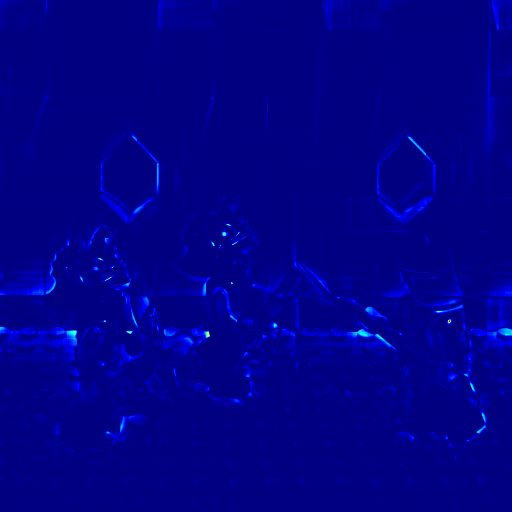
\includegraphics[height = 3.5cm]{../Figures/simulated_views/knights_tiles3x3x256x256_overlap0.5_5layers_resolution9x9x512x512_SART_50iter/MSE_for_view_(5,1).png}}\hfill%
	\subcaptionbox*{(5,5)}{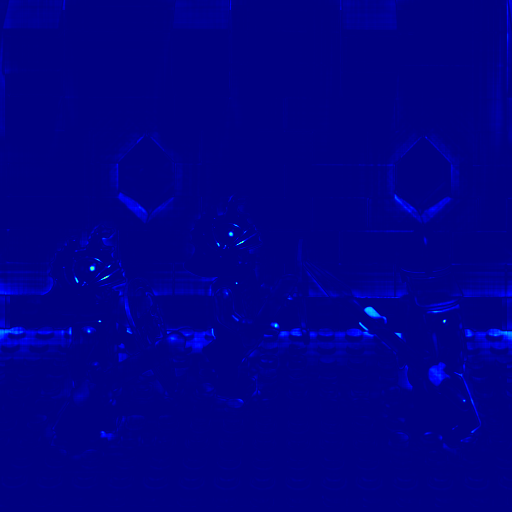
\includegraphics[height = 3.5cm]{../Figures/simulated_views/knights_tiles3x3x256x256_overlap0.5_5layers_resolution9x9x512x512_SART_50iter/MSE_for_view_(5,5).png}}\hfill%
	\subcaptionbox*{(5,9)}{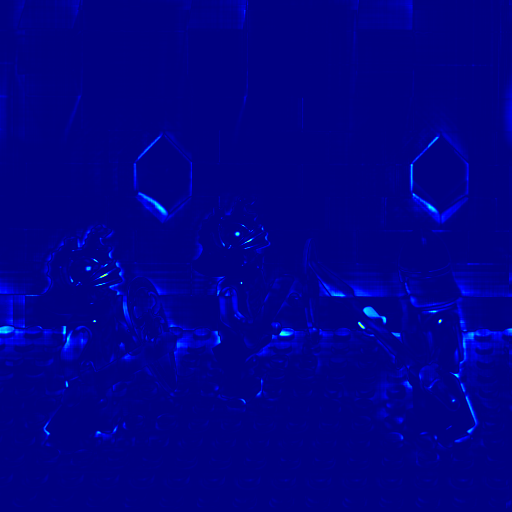
\includegraphics[height = 3.5cm]{../Figures/simulated_views/knights_tiles3x3x256x256_overlap0.5_5layers_resolution9x9x512x512_SART_50iter/MSE_for_view_(5,9).png}}
	
	\vspace{0.15cm}
	
	\subcaptionbox*{1}{
\includegraphics[height = 2.3cm]{../Figures/simulated_views/knights_tiles3x3x256x256_overlap0.5_5layers_resolution9x9x512x512_SART_50iter/1.png}}\hfill%
	\subcaptionbox*{2}{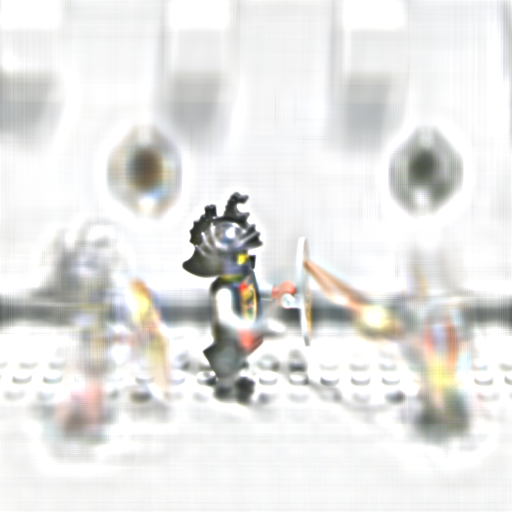
\includegraphics[height = 2.3cm]{../Figures/simulated_views/knights_tiles3x3x256x256_overlap0.5_5layers_resolution9x9x512x512_SART_50iter/2.png}}\hfill%
	\subcaptionbox*{3}{
\includegraphics[height = 2.3cm]{../Figures/simulated_views/knights_tiles3x3x256x256_overlap0.5_5layers_resolution9x9x512x512_SART_50iter/3.png}}\hfill%
	\subcaptionbox*{4}{
\includegraphics[height = 2.3cm]{../Figures/simulated_views/knights_tiles3x3x256x256_overlap0.5_5layers_resolution9x9x512x512_SART_50iter/4.png}}\hfill%
	\subcaptionbox*{5}{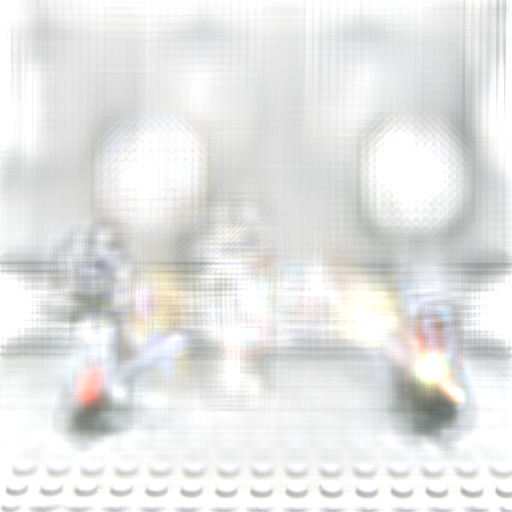
\includegraphics[height = 2.3cm]{../Figures/simulated_views/knights_tiles3x3x256x256_overlap0.5_5layers_resolution9x9x512x512_SART_50iter/5.png}}
	\caption[Simulated projections of the lego knight scene]
			{Simulated projections of the lego knight scene.
			 The light field extends over a baseline of about 14 cm with a distance of 20 cm between the two reference planes.
			 The camera plane is sampled at $9 \times 9$ positions.
			 Shown are the simulated views at different positions on the camera plane and the respective visualization of the error compared to the input light field.
			 All five attenuation layers are displayed in the bottom row.}
	\label{fig:simulated_projections_lego_knights}
\end{figure}

\begin{figure}[htb]
	\subcaptionbox*{(1,1)}{
\includegraphics[height = 3.5cm]{../Figures/simulated_views/lytro_cubes_tiles_4x4x200x200_overlap0.5_5layers_resolution_7x7x381x381_SART_50_iter/Reconstruction_of_view_(1,1).png}}\hfill%
	\subcaptionbox*{(1,4)}{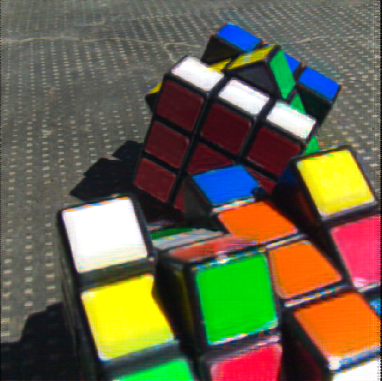
\includegraphics[height = 3.5cm]{../Figures/simulated_views/lytro_cubes_tiles_4x4x200x200_overlap0.5_5layers_resolution_7x7x381x381_SART_50_iter/Reconstruction_of_view_(1,4).png}}\hfill%
	\subcaptionbox*{(1,7)}{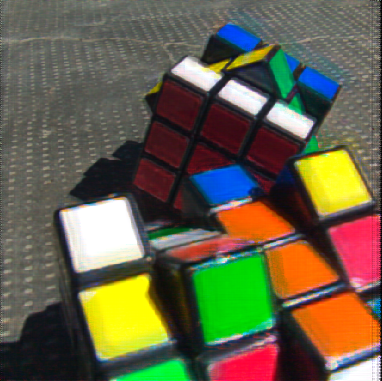
\includegraphics[height = 3.5cm]{../Figures/simulated_views/lytro_cubes_tiles_4x4x200x200_overlap0.5_5layers_resolution_7x7x381x381_SART_50_iter/Reconstruction_of_view_(1,7).png}}
	
	\vspace{0.15cm}
	
	\subcaptionbox*{(1,1)}{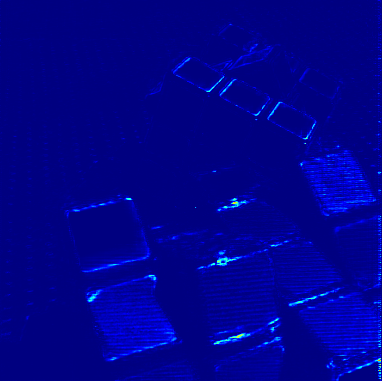
\includegraphics[height = 3.5cm]{../Figures/simulated_views/lytro_cubes_tiles_4x4x200x200_overlap0.5_5layers_resolution_7x7x381x381_SART_50_iter/MSE_for_view_(1,1).png}}\hfill%
	\subcaptionbox*{(1,4)}{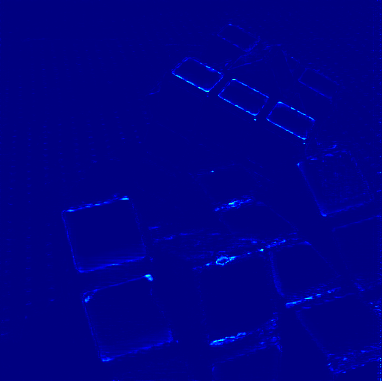
\includegraphics[height = 3.5cm]{../Figures/simulated_views/lytro_cubes_tiles_4x4x200x200_overlap0.5_5layers_resolution_7x7x381x381_SART_50_iter/MSE_for_view_(1,4).png}}\hfill%
	\subcaptionbox*{(1,7)}{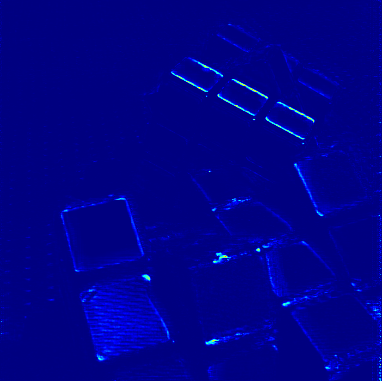
\includegraphics[height = 3.5cm]{../Figures/simulated_views/lytro_cubes_tiles_4x4x200x200_overlap0.5_5layers_resolution_7x7x381x381_SART_50_iter/MSE_for_view_(1,7).png}}
	
	\vspace{0.15cm}
	
	\subcaptionbox*{(4,1)}{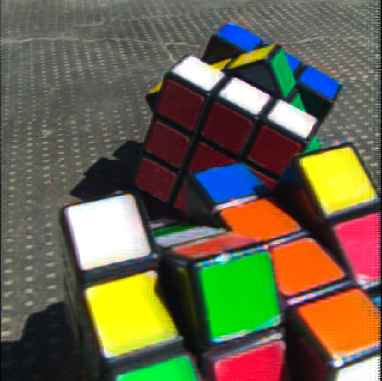
\includegraphics[height = 3.5cm]{../Figures/simulated_views/lytro_cubes_tiles_4x4x200x200_overlap0.5_5layers_resolution_7x7x381x381_SART_50_iter/Reconstruction_of_view_(4,1).png}}\hfill%
	\subcaptionbox*{(4,4)}{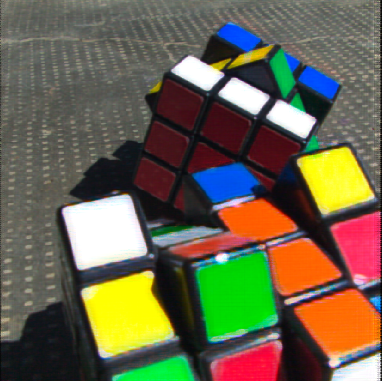
\includegraphics[height = 3.5cm]{../Figures/simulated_views/lytro_cubes_tiles_4x4x200x200_overlap0.5_5layers_resolution_7x7x381x381_SART_50_iter/Reconstruction_of_view_(4,4).png}}\hfill%
	\subcaptionbox*{(4,7)}{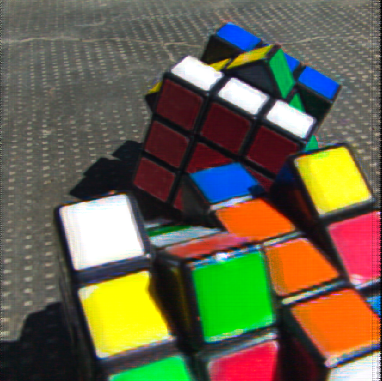
\includegraphics[height = 3.5cm]{../Figures/simulated_views/lytro_cubes_tiles_4x4x200x200_overlap0.5_5layers_resolution_7x7x381x381_SART_50_iter/Reconstruction_of_view_(4,7).png}}
	
	\vspace{0.15cm}
	
	\subcaptionbox*{(4,1)}{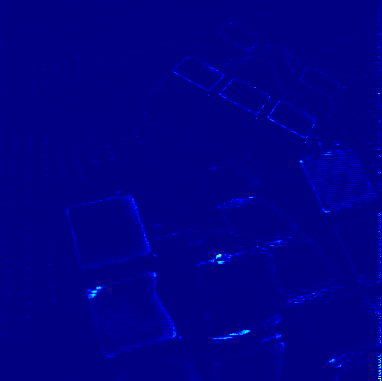
\includegraphics[height = 3.5cm]{../Figures/simulated_views/lytro_cubes_tiles_4x4x200x200_overlap0.5_5layers_resolution_7x7x381x381_SART_50_iter/MSE_for_view_(4,1).png}}\hfill%
	\subcaptionbox*{(4,4)}{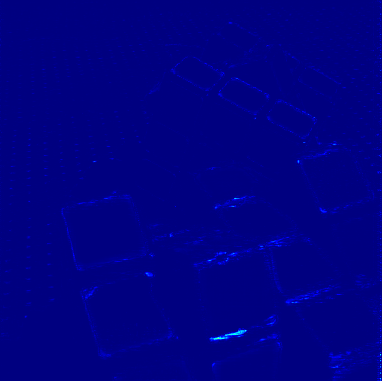
\includegraphics[height = 3.5cm]{../Figures/simulated_views/lytro_cubes_tiles_4x4x200x200_overlap0.5_5layers_resolution_7x7x381x381_SART_50_iter/MSE_for_view_(4,4).png}}\hfill%
	\subcaptionbox*{(4,7)}{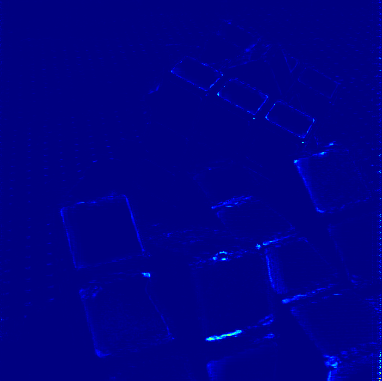
\includegraphics[height = 3.5cm]{../Figures/simulated_views/lytro_cubes_tiles_4x4x200x200_overlap0.5_5layers_resolution_7x7x381x381_SART_50_iter/MSE_for_view_(4,7).png}}
	
	\vspace{0.15cm}
	
	\subcaptionbox*{1}{
\includegraphics[height = 2.3cm]{../Figures/simulated_views/lytro_cubes_tiles_4x4x200x200_overlap0.5_5layers_resolution_7x7x381x381_SART_50_iter/1.png}}\hfill%
	\subcaptionbox*{2}{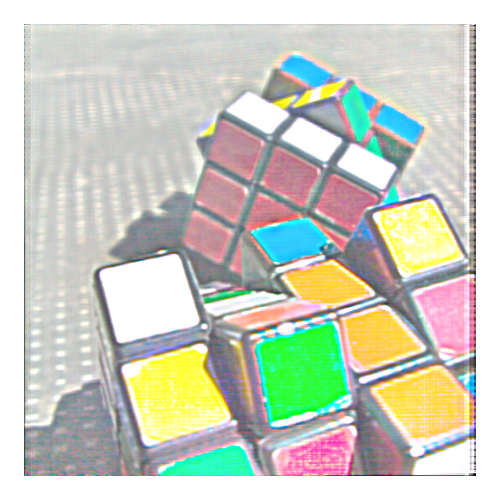
\includegraphics[height = 2.3cm]{../Figures/simulated_views/lytro_cubes_tiles_4x4x200x200_overlap0.5_5layers_resolution_7x7x381x381_SART_50_iter/2.png}}\hfill%
	\subcaptionbox*{3}{
\includegraphics[height = 2.3cm]{../Figures/simulated_views/lytro_cubes_tiles_4x4x200x200_overlap0.5_5layers_resolution_7x7x381x381_SART_50_iter/3.png}}\hfill%
	\subcaptionbox*{4}{
\includegraphics[height = 2.3cm]{../Figures/simulated_views/lytro_cubes_tiles_4x4x200x200_overlap0.5_5layers_resolution_7x7x381x381_SART_50_iter/4.png}}\hfill%
	\subcaptionbox*{5}{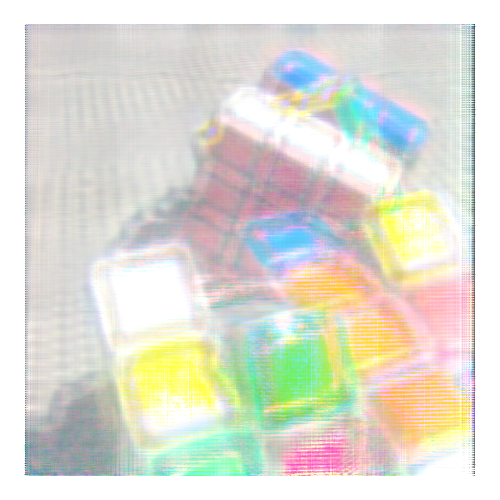
\includegraphics[height = 2.3cm]{../Figures/simulated_views/lytro_cubes_tiles_4x4x200x200_overlap0.5_5layers_resolution_7x7x381x381_SART_50_iter/5.png}}
	\caption[Simulated projections of a scene taken with Lytro]
			{Simulated projections of a scene taken with the Lytro camera.
			 The light field extends over a baseline of about 5 cm with a distance of 1 m between the two reference planes.
			 The camera plane is sampled at $7 \times 7$ positions.
			 Shown are the simulated views at different positions on the camera plane and the respective visualization of the error compared to the input light field.
			 All five attenuation layers are displayed in the bottom row.}
	\label{fig:simulated_projections_lytro_cubes}
\end{figure}
